\documentclass[11pt,paper=a4,fleqn,parskip=half% ohne Absatzeinzug
]{scrartcl}   
\usepackage[T1]{fontenc}            %% Zeichensatzkodierung fuer Silbentrennung
\usepackage[utf8]{inputenc}         %% Unicodezeichen
\usepackage[ngerman]{babel}      %% Dt. Spracheigenschaften
\usepackage{csquotes}%% \enquote{Anfuehrungszeichen}
% Schrift
\usepackage{lmodern}
\usepackage[osf,sc]{mathpazo} % Fonts to typeset mathematics to match Palatino
\usepackage{textcase}
\usepackage{nameref}
\usepackage{hyperref}
\usepackage[dvipsnames,usenames,table]{xcolor} 
\usepackage{multirow}
\usepackage{graphicx} 
\usepackage{scrhack}    
\usepackage{url}%% Links
\usepackage[inline]{enumitem}
\usepackage{pifont}
\usepackage{eurosym}% \euro 20,-
\usepackage{amsmath}
\usepackage{amsfonts}
\usepackage{amssymb}
\usepackage{array}            % Extending the array and tabular environments
\usepackage{chngcntr}         % Change the resetting of counters
\usepackage[version=4]{mhchem}
\usepackage{stmaryrd}
\usepackage{siunitx}
\usepackage{float}
\usepackage{multicol}
\usepackage{caption, booktabs}

% eigene Farbe definieren
% Adobe Prozessfarben: CMYK: 100,50,0,35 -> 1,0.5,0,0.35
\definecolor{orange}{cmyk}{0,0.55,0.61,0}   % 0,55,61,0
\definecolor{blau5}{cmyk}{1,0.77,0.1,0.01}  % 100,77,10,
\definecolor{rot5}{cmyk}{0.22,1,1,0.19}   % 22,100,100,19
\definecolor{grau2}{cmyk}{0,0,0,0.4}          % 0,0,0,40

\usepackage[headsepline,automark]{scrlayer-scrpage} 
% headings
\pagestyle{scrheadings}
\automark*[section]{}

\usepackage{latexsym}   % to get the \Box symbol
\usepackage{footnote}
\usepackage{qrcode}% Anwendung: \qrcode[hyperlink,level=Q,version=2,height=1cm]{\website}
\usepackage{underscore}% Unterstrich ____
% PDF Dokumente einbinden
\usepackage{pdfpages}% \includepdf[pages=-]{Tabellen/Inventar-1}

% bibliography
\usepackage[
    bibencoding=utf8,
    backend=biber,% bibtex, biber
    backref=false,backrefstyle=three+,url=true,urldate=comp,abbreviate=false,maxnames=20
]{biblatex} %Paket laden
\DeclareBibliographyCategory{cited}
\let\defaultcite\cite\renewcommand*\cite[2][]{\addtocategory{cited}{#2}\defaultcite[#1]{#2}}
\let\defaulttextcite\textcite\renewcommand*\textcite[2][]{\addtocategory{cited}{#2}\defaulttextcite[#1]{#2}}
\setcounter{biburllcpenalty}{7000}
\setcounter{biburlucpenalty}{8000}
\AfterPackage{biblatex}{
	\PreventPackageFromLoading[\errmessage{Sie haben versucht, das Cite-Paket zu laden, das nicht mit biblatex kompatibel ist.}]{cite}
}


% listings
\usepackage{listings}
\lstset{basicstyle=\linespread{1}\ttfamily\small,floatplacement=!htb,captionpos=t,abovecaptionskip=.5\baselineskip,belowcaptionskip=.5\baselineskip,upquote=true,showstringspaces=false,inputencoding=utf8,tabsize=4,
    keywordstyle=\bfseries \color{black},
	commentstyle=\color{rot5},
	%stringstyle=\color{orange},
	breaklines=true,
  	postbreak=\mbox{\textcolor{rot5}{$\hookrightarrow$}\space},
	breakatwhitespace=false
}
\lstset{literate={á}{{\'a}}1 {é}{{\'e}}1 {í}{{\'i}}1 {ó}{{\'o}}1 {ú}{{\'u}}1 {Á}{{\'A}}1 {É}{{\'E}}1 {Í}{{\'I}}1 {Ó}{{\'O}}1 {Ú}{{\'U}}1 {à}{{\`a}}1 {è}{{\`e}}1 {ì}{{\`i}}1 {ò}{{\`o}}1 {ù}{{\`u}}1 {À}{{\`A}}1 {È}{{\'E}}1 {Ì}{{\`I}}1 {Ò}{{\`O}}1 {Ù}{{\`U}}1 {ä}{{\"a}}1 {ë}{{\"e}}1 {ï}{{\"i}}1 {ö}{{\"o}}1 {ü}{{\"u}}1 {Ä}{{\"A}}1 {Ë}{{\"E}}1 {Ï}{{\"I}}1 {Ö}{{\"O}}1 {Ü}{{\"U}}1 {â}{{\^a}}1 {ê}{{\^e}}1 {î}{{\^i}}1 {ô}{{\^o}}1 {û}{{\^u}}1 {Â}{{\^A}}1 {Ê}{{\^E}}1 {Î}{{\^I}}1 {Ô}{{\^O}}1 {Û}{{\^U}}1 {œ}{{\oe}}1 {Œ}{{\OE}}1 {æ}{{\ae}}1 {Æ}{{\AE}}1 {ß}{{\ss}}1 {ű}{{\H{u}}}1 {Ű}{{\H{U}}}1 {ő}{{\H{o}}}1 {Ő}{{\H{O}}}1 {ç}{{\c c}}1 {Ç}{{\c C}}1 {ø}{{\o}}1 {å}{{\r a}}1 {Å}{{\r A}}1 {€}{{\EUR}}1 {£}{{\pounds}}1 {~}{{\textasciitilde}}1 {-}{{-}}1 }

\hypersetup{%
	%pdftitle={\titel},
	%pdfsubject={Latex},
	%pdfauthor={\autor},
	%pdfcreator={\autor}, 
	bookmarksnumbered=true,
	breaklinks=true,
	%colorlinks=true,	   
	linkcolor=rot5,		
	filecolor=blau5,		
	urlcolor=blau5,			
	citecolor=ForestGreen
}

%\AtBeginDocument{\recalctypearea}
\linespread{1.1}
\setlist{itemsep=0pt}
\widowpenalty10000
\clubpenalty10000
\tolerance1000    
%%%%%%%%%%%%%%%%%%%%%%%%%%%%%%%%%%%%%%%%%%%%%%%%%%%%%%%%%%%%%%%%%%%
% Eingabe
% Seitenlayout
\usepackage[left=2.0cm,right=2.0cm,top=2.0cm,bottom=2.0cm,includeheadfoot]{geometry}
\setlength{\footheight}{28.45268pt}
\setlength{\headheight}{33.16006pt}



% Kopfzeile
\ihead{\copyright \enspace $\the\year$ \autor\\ \small{\textbf{Quelle:} \quelle} \vspace{0.4em}}
\chead{}%leer lassen
% mit Logo & QR-Code????
\ohead{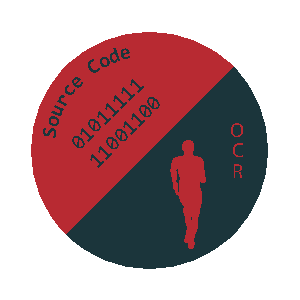
\includegraphics[width=1.0cm]{images/logo.eps}}% Logo
\ifoot{\qrcode[hyperlink,level=Q,version=2,height=1.0cm]{\website}}% QR-Code

% anpassen
% Quelle Literaturverzeichnis oder URL in Fussnote 
\newcommand{\quelle}{Jan Schaffranek franneck94~\footnote{\url{https://github.com/franneck94}}}
%\newcommand{\quelle}{MathePeter siehe~\textcite{peter:2021:mathe}}% Literaturverzeichnis
\newcommand{\titel}{Python Notizen}
\newcommand{\autor}{Jan Unger}
\newcommand{\datum}{\today}
\newcommand{\datumHand}{09.07.2021}% ##.##.####
\newcommand{\website}{http://bw-ju.de}
\newcommand{\websiteKurz}{bw-ju.de}



% Literatur
\bibliography{content/literatur}
\bibliography{content/literatur-kfz}
\bibliography{content/literatur-sport}


%%%%%%%%%%%%%%%%%%%%%%%%%%%%%%%%%%%%%%%%%%%%%%%%%%%%%%%%%%%%%%%%%%
% \LaTeX
% \begin{enumerate}[label=(\alph*)]% (a)
% \begin{itemize}[label=\checkmark]% check
% \begin{enumerate}[label={\protect\ding{\value*}},start=192]% (1)
% \textbf{fetter Text}
% \textsc{Kapitaelchen}
% \emph{kursiv}
% \enspace % Abstand oder \quad
% \huge{großer Text}
% \tiny{kleiner Text}
% \textcolor{rot5}{farbiger Text \LaTeX}

%\title{\titel}
%\date{\datum}
%\author{\autor}

\begin{document}

    %\maketitle
    % oder
    \begin{center}
        \textbf{\Large \titel}\\%14pt
        \vspace{0.4em}
        \datum
        %\datumHand
    \end{center}

    %%%%%%%%%%%%%%%%%%%%%%%%%%%%%%%%%%%%%%%%%%%%%%%%%%%%%%%%%%%%%%%%%%
    % Zusammenfassung anpassen
    \begin{abstract} 
    \begin{quote}
        \textcolor{rot5}{>>Die Mathematik ist die Sprache der Natur, 
        ihre Buchstaben sind Dreiecke, Kreise und andere Figuren.<<}\\ 
        \raggedleft \small{-- Galileo Galilei}% 10pt
    \end{quote}
    \end{abstract}

    % Check anpassen
    \begin{itemize}[label=\checkmark] \itemsep -2pt
        \item keywords
    \end{itemize}

    % Textteil anpassen

    %Fußnote~\footnote{Text der Fußnote.} 

    %\textbf{Quelle:} \quelle

    %Meine Website~\footnote{\url{\website}}


    %ju 22-Jul-21 keywords.tex
\section{boolean true false}\label{boolean-true-false}

\lstset{language=Python}% C, TeX, Bash, Python 
\begin{lstlisting}[
	%caption={}, label={code:}%% anpassen
][language=Python]
# boolean true, false
log_var1 = True == (1 > 2) # False
log_var2 = True == (2 > 1) # True
\end{lstlisting}

\section{and or not}\label{and-or-not}

\lstset{language=Python}% C, TeX, Bash, Python 
\begin{lstlisting}[
	%caption={}, label={code:}%% anpassen
][language=Python]
# and, or, not
log_var3 = True and True # True
log_var4 = True or False # True
log_var5 = not False # True
\end{lstlisting}

\section{break continue}\label{break-continue}

\lstset{language=Python}% C, TeX, Bash, Python 
\begin{lstlisting}[
	%caption={}, label={code:}%% anpassen
][language=Python]
# break, continue
while True:
    break    # ende
    continue # abbruch
\end{lstlisting}

\section{class}\label{class}

\lstset{language=Python}% C, TeX, Bash, Python 
\begin{lstlisting}[
	%caption={}, label={code:}%% anpassen
][language=Python]
# class
#class Coffee:
    # Define your class
\end{lstlisting}

\section{funktion}\label{funktion}

\lstset{language=Python}% C, TeX, Bash, Python 
\begin{lstlisting}[
	%caption={}, label={code:}%% anpassen
][language=Python]
def say_hi():
    print("hi")


say_hi()
\end{lstlisting}

\section{if elif else}\label{if-elif-else}

\lstset{language=Python}% C, TeX, Bash, Python 
\begin{lstlisting}[
	%caption={}, label={code:}%% anpassen
][language=Python]
x = int(input("Eingabe Zahl: "))
if x > 3: print("Big")
elif x == 3: print("3")
else: print("Small")
\end{lstlisting}

\section{for while}\label{for-while}

\lstset{language=Python}% C, TeX, Bash, Python 
\begin{lstlisting}[
	%caption={}, label={code:}%% anpassen
][language=Python]
# For 
for i in [0,1,2]:
    print(i)

# While 
j = 0
while j < 3:
    print(j); j = j + 1
\end{lstlisting}

\section{in}\label{in}

\lstset{language=Python}% C, TeX, Bash, Python 
\begin{lstlisting}[
	%caption={}, label={code:}%% anpassen
][language=Python]
# in
liste = [2, 39, 42]
log_var6 = 42 in liste # True
log_var6
\end{lstlisting}

\section{is}\label{is}

\lstset{language=Python}% C, TeX, Bash, Python 
\begin{lstlisting}[
	%caption={}, label={code:}%% anpassen
][language=Python]
# is
y = x = 3
log_var7 = x is y # True
\end{lstlisting}

\section{None}\label{none}

\lstset{language=Python}% C, TeX, Bash, Python 
\begin{lstlisting}[
	%caption={}, label={code:}%% anpassen
][language=Python]
# None
print() is None # True
\end{lstlisting}

\section{lambda}\label{lambda}

\lstset{language=Python}% C, TeX, Bash, Python 
\begin{lstlisting}[
	%caption={}, label={code:}%% anpassen
][language=Python]
# lambda
(lambda x: x+3)(2) # 5
\end{lstlisting}

\section{return}\label{return}

\lstset{language=Python}% C, TeX, Bash, Python 
\begin{lstlisting}[
	%caption={}, label={code:}%% anpassen
][language=Python]
# return
def increment(x):
    return x + 1

    
increment(4) # returns 5
\end{lstlisting}

    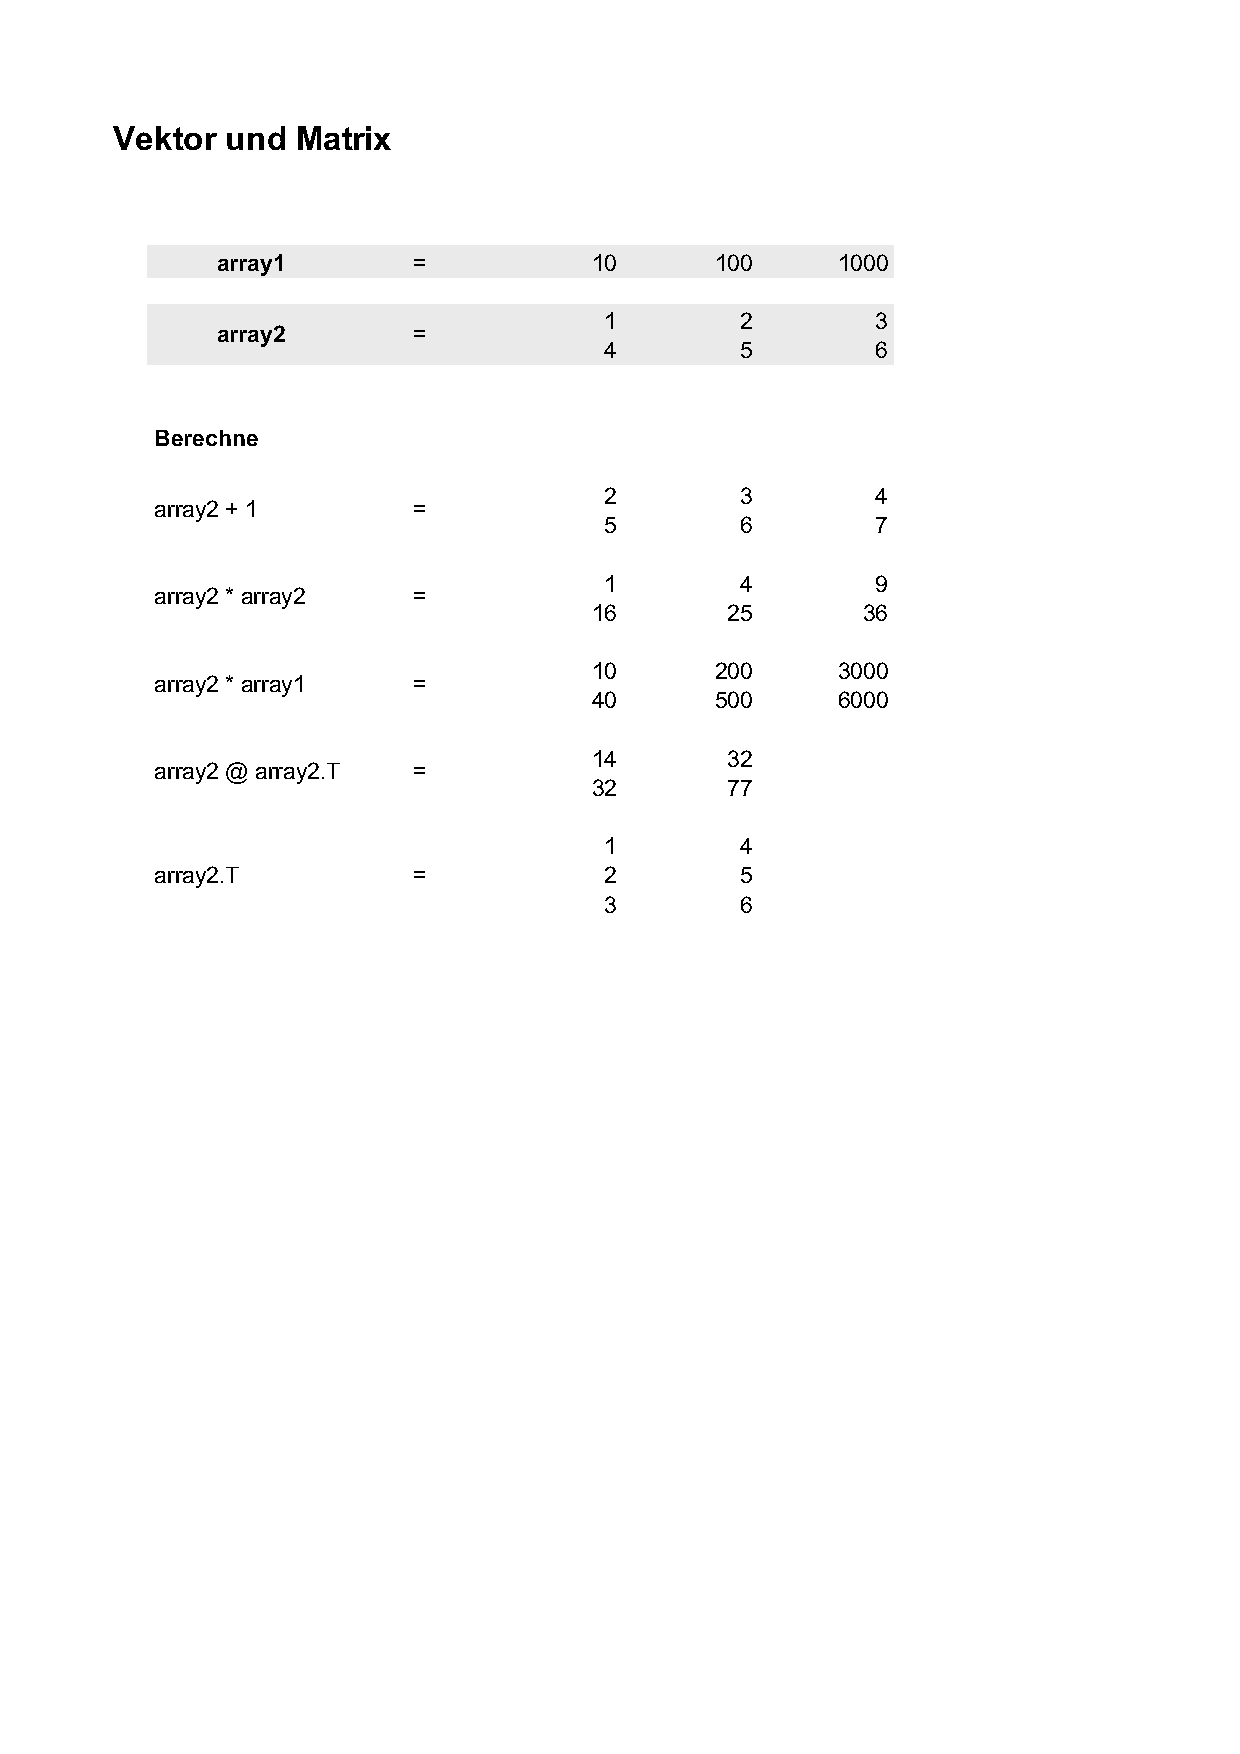
\includepdf[pages=-]{Tabellen/PDF/Vektor-und-Matrix.pdf}     
    %%ju 22-Jul-21 Neu.tex
Neuer Inhalt
 % neu

    %%%%%%%%%%%%%%%%%%%%%%%%%%%%%%%%%%%%%%%%%%%%%%%%%%%%%%%%%%%%%%%%%%
    % Bibliographie
    \printbibliography

\end{document}